\section{Cel pracy}
Celem pracy jest analiza możliwych sposobów definiowania typów ilorazowych w Coqu. Skupimy się jednak jedynie na typach ilorazowych, dla których istnieje funkcja normalizująca. Dodatkowo zostanie przedstawione dla których typów można zdefiniować taką funkcję, a dla których jest to nie możliwe. Koncentrować przy tym będziemy się na podejściu wykorzystującym zdefiniowany w bibliotece standardowej Coqa predykat równości, nie wykorzystując dodatkowych aksjomatów. Zostaną natomiast pokazane jakie możliwość dawałoby ich wykorzystanie w odpowiednich konstrukcjach. Gdyż język Coq nie posiada wsparcia dla typów ilorazowych będziemy musieli wykorzystać inne techniki pozwalające na pracę podobną do pracy z typami ilorazowymi. Głównym tematem zainteresowania tej pracy są typy indykatywne które pozwalając na jednoznaczną reprezentację danego typu ilorazowego, oraz ich tworzenie na podstawie funkcji normalizujących tych że typów. 

\section{Czym jest Coq?}
Coq jest darmowym asystentem dowodzenia na licencji GNU LGPL. Jego pierwsza wersja powstała w 1984 roku jako implementacja bazującego na teorii typów rachunku konstrukcji (Calculus of Constructions). Od 1991 roku Coq wykorzytsuje bardziej zaawansowany rachunek indukcyjnych konstrukcji (Calculus of Inductive Constructions)\cite{cic}, który pozwala zarówno na logikę wyższego rzędu, jak i na statycznie typowane funkcyjne programowanie, wszystko dzięki izomorfizmowi Curry'ego - Howarda \cite{curry-howard}. Coq pozwala na proste obliczenia, lecz jest przygotowany pod ekstrakcję już gotowych programów do innych języków funkcyjnych, jakich jak OCaml. W Coqu każdy term ma swój typ, a każdy typ ma swoje uniwersum:
\begin{description}
    \item[\mintinline{coq}{Prop}] - jest to uniwersum twierdzeń. Jest ono niepredykatatywne co pozwala na tworzenie zdań, które coś mówią o innych zadnich. To uniwersum jest usuwane podczas ekstrakcji kodu, przez co nie możliwym jest dopasowywanie do wzorca dowodów twierdzeń podczas konstrukcji typów, z wyjątkiem konstrukcji mających tylko jedno trywialne dopasowanie.
    \item[\mintinline{coq}{SProp}] - to samo co \mintinline{coq}{Prop} zawierające jednak dodatkowo definicyjną irrelewancję dowodów, czyli wszystkie dowody tego samego twierdzenie są z definicji tym samym dowodem.
    \item[\mintinline{coq}{Set}] - jest to predykatywne uniwersum przeznaczone dla obliczeń. Jest ono zachowywane podczas ekstrakcji kodu.
    \item[\mintinline{coq}{Type}] - jest to nad uniwersum pozostałych, czyli \mintinline{coq}{Prop : Type} itp. Tak naprawdę uniwersów \mintinline{coq}{Type} jest nieskończenie wiele, gdyż każde uniwersum nie może zawierać same siebie, przez co  \mintinline{coq}{Type(i) : Type (i+1)}.
\end{description}
Coq pozwala jedynie na definiowanie funkcji które terminują, co czyni z niego język nie równoważny maszynie Turinga, jednak w dalszej części pracy pokażemy jak modelować nie terminujące obliczenia w Coqu. Główną zaletą Coqa jest jednak możliwość pisania dowodów (jak i programów) za pomocą gotowych taktyk, oraz możliwość interaktywnego przyglądania się które części dowodu wymagają jeszcze udowodnienie. Pozwala to na dużo łatwiejsze dowodzenie niż w językach takich jak Idris czy Agda.
\section{Czym są typy ilorazowe}
W algebrze abstrakcyjnej zbiór pierwotny $T$, w którym utożsamiamy elementy zgodnie z relacją równoważności $(\sim)$ nazywamy strukturą ilorazową. Oznaczmy ją symbolem $T/\sim$. Dobrym przykładem tego typu struktury jest grupa z modularną arytmetyką. Każdy z nas zaznajomiony z zasadami działania zegara i nikogo nie dziwni że po godzinie dwunastej następuje godzina pierwsza. O godzinach na traczy zegara możemy myśleć jako o operacjach w grupie $\mathbb{Z} / 12\mathbb{Z}$, czyli takiej, w której utożsamiamy liczby których operacja dzielenia przez 12 daje taką samą resztę.
\begin{equation}
\dots 	\equiv -11 	\equiv 1 \equiv 13 \equiv 25 \equiv 37 \equiv \dots \;\;(\textrm{mod } 12)
\label{mod_12}
\end{equation}
Tak jak podpowiada nam intuicja 1:00 i 13:00 to ta sama godzina w tej arytmetyce.
\subsection{Relacja równoważności}
Żeby sformalizować typy ilorazowe, będziemy usieli najpierw dokładnie zdefiniować jakie relacje są relacjami równoważności. Każda relacja równoważności spełnia trzy własności:
\begin{description}
    \item[Zwrotność] - każdy element musi być w relacji sam z sobą ($a \sim a$)
    \item[Symetryczność] - jeśli $a$ jest w relacji z $b$ ($a \sim b$) to również relacja zachodzi w odwrotnej kolejności  ($b \sim a$).
    \item[Przechodniość] - jeśli istnieje punkt $b$ z którym zarówno $a$ i $c$ są w relacji (odpowiednio $a \sim b$ oraz $b \sim c$) to $a$ jest w relacji z $c$ ($a \sim c$).
\end{description}
\begin{code}
\begin{minted}{coq}
Class equivalance_relation {A: Type} (R: A -> A -> Prop) := {
  equiv_refl  : forall x: A, R x x;
  equiv_sym   : forall x y: A, R x y -> R y x;
  equiv_trans : forall x y z: A, R x y -> R y z -> R x z;
}.
\end{minted}
\caption{Klasa relacji równoważności zapisana w Coq}
\label{equivalance_relation}
\end{code}
Najlepszym przykładem takiej relacji jest równość, po chwili zastanowienie widać iż spełnia ona wszystkie trzy wymagane własności. O relacjach równoważności możemy myśleć jako o uogólnieniu pierwotnego pojęcia równości elementów. Pozwalają one na utożsamienie różnych elementów naszego pierwotnego zbioru z sobą np. godzinę 13:00 z 1:00. Innym przykładem może być utożsamienie różnych reprezentacji tej samej liczby $\frac{1}{2}$ z $\frac{2}{4}$. Z punktu widzenia teorii mnogości utożsamione z sobą elementy tworzą klasy abstrakcji. Tak naprawdę w tej teorii $T/\sim$ jest rodziną klas abstrakcji, inaczej mówiąc rodziną zbiorów elementów które zostały utożsamione relacją ($\sim$).

\begin{figure}[!htp]
    \centering
    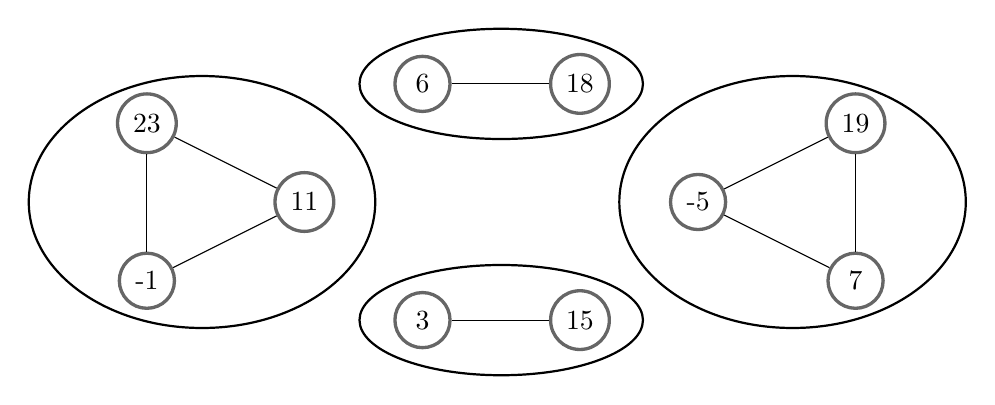
\begin{tikzpicture}[
    node/.style={circle, draw=black!60, very thick, minimum size=7mm},
    ]
    %Nodes
    \node[node] at (-0.5, 0.5) (a) {-1};
    \node[node] at (1.5, 1.5) (b) {11};
    \node[node] at (-0.5, 2.5) (c) {23};
    \node[node] at (6.5, 1.5) (d) {-5};
    \node[node] at (8.5, 0.5) (e) {7};
    \node[node] at (8.5, 2.5) (f) {19};
    \node[node] at (3, 0) (g) {3};
    \node[node] at (5, 0) (h) {15};
    \node[node] at (3, 3) (i) {6};
    \node[node] at (5, 3) (j) {18};
    
    %Lines
    \draw[-] (a) -- (b);
    \draw[-] (a) -- (c);
    \draw[-] (b) -- (c);
    \draw[-] (d) -- (e);
    \draw[-] (d) -- (f);
    \draw[-] (e) -- (f);
    \draw[-] (g) -- (h);
    \draw[-] (i) -- (j);
    
    %elipses
    \draw[thick] (4,0) ellipse (1.8 and 0.7);
    \draw[thick] (4,3) ellipse (1.8 and 0.7);
    \draw[thick] (0.2,1.5) ellipse (2.2 and 1.6);
    \draw[thick] (7.7,1.5) ellipse (2.2 and 1.6);
    \end{tikzpicture}
    \caption{Przykład elementów utożsamionych z sobą w grupie $\mathbb{Z} / 12\mathbb{Z}$, linie oznaczają elementy będące z sobą w relacji równoważności, a elipsy klasy abstrakcji wyznaczone przez tą relację równoważności}
    \label{fig:fourier_vis}
\end{figure}


\subsection{Spojrzenie teorii typów}
Jako że praca skupia się na implementacji typów ilorazowych w Coqu, stąd też bardziej skupimy się na spojrzeniu teorii typów na ilorazy, w przeciwieństwie do spojrzenia teorio mnogościowego. W teorii typów $T/\sim$ będziemy nazywać typem ilorazowym generowanym przez relację równoważności $(\sim)$ na typie pierwotnym $T$. Będziemy oznaczać $a = b$ w typie $T/\sim$ wtedy i tylko wtedy gdy $a \sim b$. Widzimy zatem iż każdy element typ $T$ jest również elementem typu $T/\sim$. Natomiast nie wszystkie funkcje z typu $T$ są dobrze zdefiniowanymi funkcjami z typu $T/\sim$. Funkcja $f: T \rightarrow X$ jest dobrze zdefiniowaną funkcją $f: (T/\sim) \rightarrow X$ jeśli spełnia warunek, że $a \sim b$ implikuje $f(a) = f(b)$. Ten warunek jest konieczny, aby nie dało się rozróżnić utożsamionych wcześniej elementów poprzez zmapowanie ich do innego typu. Myśląc o wszystkich elementach będących z sobą w relacji $(\sim)$ jako o jednym elemencie brak tej zasady spowodowałby złamanie reguły monotoniczności aplikacji mówiącej, że $x = y \Rightarrow f (x) = f (y)$.
\section{Relacje równoważności generowane przez funkcję normalizującą}
Każda funkcja $h: T \rightarrow B$ generuje nam pewną relację równoważności ($\sim_h$) zdefiniowaną poniżej:
\begin{equation}
    \forall x, y \in T, x \sim_h y \iff h(x) = h(y)
\end{equation}
Jak już wspominaliśmy równość jest relacją równoważności, stąd łatwo pokazać iż ($\sim_h$) jest relacją równoważności. Dowolna funkcja $g: B \rightarrow X$ będzie teraz generować dobrze zdefiniowaną funkcję $f: T /\sim_h \rightarrow X$ w taki sposób, że $f = g \circ h$.
\subsection{Funkcja normalizująca}
W tej pracy skupimy się na szczególnym przypadku funkcji $h: T \rightarrow B$ w którym $B = T$. Dodatkowo będziemy wymagać aby funkcja $h$ była idempotentna. Tak zdefiniowaną funkcję h będziemy nazywać funkcją normalizującą.
\begin{code}
\begin{minted}{coq}
Class normalizing_function {A: Type} (f: A -> A) := 
  idempotent : forall x: A, f (f x) = f x.
\end{minted}
\caption{Klasa funkcji normalizujących}
\label{normalizing_function}
\end{code}
Zbudujmy jeszcze odrobinę intuicji wokół tak zdefiniowanych funkcji normalizujących. Jak wiemy relacja równoważności łączny utożsamiane z sobą elementy w grupy, a mówiąc ściślej klasy abstrakcji. Celem funkcji normalizujących jest wyznaczenie reprezentanta każdej z klas abstrakcji. Obrazem tej funkcji będzie właśnie zbór naszych reprezentantów lub inaczej elementów w postaci normalnej. Warunek idempotencji jest konieczny do tego aby obrazem elementu w postaci normalnej był on sam, gdyż nie wymaga on już normalizacji.

\begin{figure}[!htp]
    \centering
    \begin{tikzpicture}[
    node/.style={circle, draw=black!60, very thick, minimum size=0.4}
    ]
    
    %Nodes
    \node[node, double] at (2, 2) (a) {$\frac{1}{2}$};
    \node[node] at (0.5, 3.5) (a0) {$\frac{2}{4}$};
    \node[node] at (3.5, 3.5) (a1) {$\frac{3}{6}$};
    \node[node] at (0.5, 0.5) (a2) {$\frac{10}{20}$};
    \node[node] at (3.5, 0.5) (a3) {$\frac{20}{40}$};

    \node[node, double] at (9, 2) (b) {$\frac{1}{3}$};
    \node[node] at (11.1, 2) (b1) {$\frac{2}{6}$};
    \node[node] at (6.9, 2) (b2) {$\frac{3}{9}$};
    \node[node] at (7.95, 0.2) (b3) {$\frac{4}{12}$};
    \node[node] at (7.95, 3.8) (b4) {$\frac{5}{15}$};
    \node[node] at (10.05, 0.2) (b5) {$\frac{10}{30}$};
    \node[node] at (10.05, 3.8) (b6) {$\frac{6}{18}$};
    
    %Lines
    \path[->, thick] (a) edge [loop above] node {};
    \draw[->, thick] (a0) -- (a);
    \draw[->, thick] (a1) -- (a);
    \draw[->, thick] (a2) -- (a);
    \draw[->, thick] (a3) -- (a);
    
    \path[->, thick] (b) edge [loop above] node {};
    \draw[->, thick] (b1) -- (b);
    \draw[->, thick] (b2) -- (b);
    \draw[->, thick] (b3) -- (b);
    \draw[->, thick] (b4) -- (b);
    \draw[->, thick] (b5) -- (b);
    \draw[->, thick] (b6) -- (b);
    \end{tikzpicture}
    \caption{Przykład działania funkcji normalizującej dla reprezentacji liczby wymiernych w postaci $\mathbb{Z} \times \mathbb{N}$}
    \label{fig:normalizing_function}
\end{figure}

\subsection{Przykłady funkcji normalizujących}
Wykorzystajmy tutaj już wcześniej przytoczony przykład liczb wymiernych. Jednym z sposobów na zdefiniowanie postaci normalnej liczby wymiernej rozumianej jako $\mathbb{Z} \times \mathbb{N}$ jest wymuszenie, aby licznik był względnie pierwszy z mianownikiem. Wprawne oko zapewne zauważy, iż $0$ nie ma kanonicznej postawi w takiej definicji, ale możemy arbitralnie ustalić, że jego postacią normalną będzie $\frac{0}{1}$. W takim przypadku funkcja normalizująca powinna dzielić licznik i mianownik przez ich największy wspólny dzielnik.
W przypadku par nieuporządkowanych, ale na których istnieje jakiś porządek liniowy postacią normalną może być para uporządkowana w której mniejszy element występuje na początku, a funkcją normalizującą będzie funkcja sortująca dwa elementy. Ostatnim, a zarazem najprostszym przykładem niech będzie postać normalna elementów w arytmetyce modularnej o podstawie $m$. Tutaj sama operacja będzie naszą funkcją normalizującą, a więc zostawimy jedynie elementy od zera do $m-1$.   
\section{Typy ilorazowe nie posiadające funkcji normalizujących}
Wykorzystanie funkcji normalizujących w definicji typów ilorazowych jest bardzo wygodne z względu na fakt, że może posłużyć nam do ograniczenia liczby reprezentantów danej klasy abstrakcji do tylko jednego, tego który jest w postaci normalnej. Problem jest jednak to, iż nie każdy typ ilorazowy posiada taką funkcję. W teorii mnogości z aksjomatem wyboru, możemy zawsze wykorzystać ów aksjomat mówiący o tym że z każdej rodziny niepustych zbiorów możemy wybrać zbiór selektorów, w naszym przypadku zbiór elementów w postaci normalnej. Niestety nie możemy skorzystać z niego w Coqowym rachunku indykatywnych konstrukcji. Zobaczmy zatem jakie typy ilorazowe nie są definiowalne w ten sposób
\subsection{Para nieuporządkowana}
Jest to najprostszy typ którego nie można zdefiniować w ten sposób. W żaden sposób nie można określić czy para $\{	\square, \medcircle \}$ jest w postaci normalnej, a może $\{ \medcircle , \square \}$. Oczywiście mając parę wartości na której istnieje pewien porządek zupełny możemy w zbudować parę wykorzystując go. Niestety w ogólności jest to niemożliwe. Niestety wraz z tym idzie iż zbiory, jak i multi-zbiory również nie mają w ogólności swoich postaci kanonicznych, a więc nie można ich zdefiniować dla typów nieposiadających w tym przypadku porządku liniowego.
\subsection{Liczby rzeczywiste definiowane za pomocą ciągów Cauchy'eago}
Kolejnym typem który w spodziewany sposób nie da się znormalizować są liczby rzeczywiste. W Coqu najlepiej je zdefiniować za pomocą ciągów Cauchy'eago liczb wymiernych.
\begin{equation}
    \textbf{isCauchy}(f) := \forall m, n \in \mathbb{N}^+, n < m \rightarrow |f_n - f_m| < \frac{1}{n}
\end{equation}
Granice ciągu będą wyznaczać, którą liczbę rzeczywistą reprezentuje dany ciąg. Chcielibyśmy zatem, aby ciągi o tej samej granicy były z sobą w relacji równoważności. Wyznaczenie granicy ciągu mając jedynie czarną skrzynkę, która może jedynie wyliczać kolejne jej elementy jest niemożliwe. Załóżmy, że jednak jest możliwe, niech $s_k$ będzie ciągiem 1 do k-tego miejsca a później stałym ciągiem 0, natomiast $s_\infty$ ciągiem samych 1. Problem sprawdzenia równości tych ciągów jest przeliczanie rekurencyjny (ciąg $s_k$ może reprezentować zatrzymanie działania programu w $k$-tej sekundzie). Oba ciągi mają różne granice, a co za tym idzie powinny mieć różne postacie normalne, a więc istnieje jakiś element na którym się różnią. Gdyby istniała zatem taka obliczalna i całkowita funkcja normalizująca moglibyśmy za jej pomocą rozwiązać problem stopu w rekurencyjny sposób, sprawdzając jedną wartość ciągu w postaci normalnej. Zatem nie może istnieć taka funkcja.
\subsection{Monada częściowych obliczeń}
Kolejnym typem ilorazowym, dla którego nie może istnieć funkcja normalizująca jest typ częściowych obliczeń. Jak widzimy w definicji \ref{deleyed} jest to typ coinduktywny produkujący albo wynik działania funkcji, albo dalsze obliczenia, które mogą, ale nie muszą się kiedyś skończyć.
\begin{code}
\begin{minted}{coq}
CoInductive delayed (A : Type) := Delayed {
  state : A + delayed A
}.
\end{minted}
\caption{Definicja monady częściowych obliczeń w Coqu.}
\label{deleyed}
\end{code}
W relacji równoważności chcielibyśmy aby były wszystkie obliczenia które ostatecznie zwrócą ten sam wynik, naturalnie będzie istnieć osobna klasa abstrakcji dla obliczeń, które nigdy się nie skończą. Podobnie jednak jak w przypadku powyżej pomimo iż możemy dla każdej klasy abstrakcji wyznaczyć jej reprezentanta w łatwy sposób (obliczenie które natychmiast zwraca wynik), to nie jest to funkcja całkowita rekurencyjna. Możemy zauważyć że za pomocą monady częściowych obliczeń możemy reprezentować dowolne obliczenia wykonywane na maszynie Turinga. Gdyby zatem potrafiliśmy w skończonym czasie wyznaczyć reprezentanta dla każdych obliczeń moglibyśmy w skończonym czasie stwierdzić czy maszyna Turinga się kiedyś zatrzyma, czy też nie. Oznaczało by to rozwiązanie problemu stopu, który jak wiem jest problemem nie rekurencyjnym. 

